\documentclass[border=10pt]{standalone}

\usepackage{tikz}
\usepackage{tikzsymbols}
\usetikzlibrary{calc,patterns,shapes.geometric}

\def\centerarc[#1](#2)(#3:#4:#5){\draw[#1] ($(#2)+({#5*cos(#3)},{#5*sin(#3)})$) arc (#3:#4:#5);}

\begin{document}
	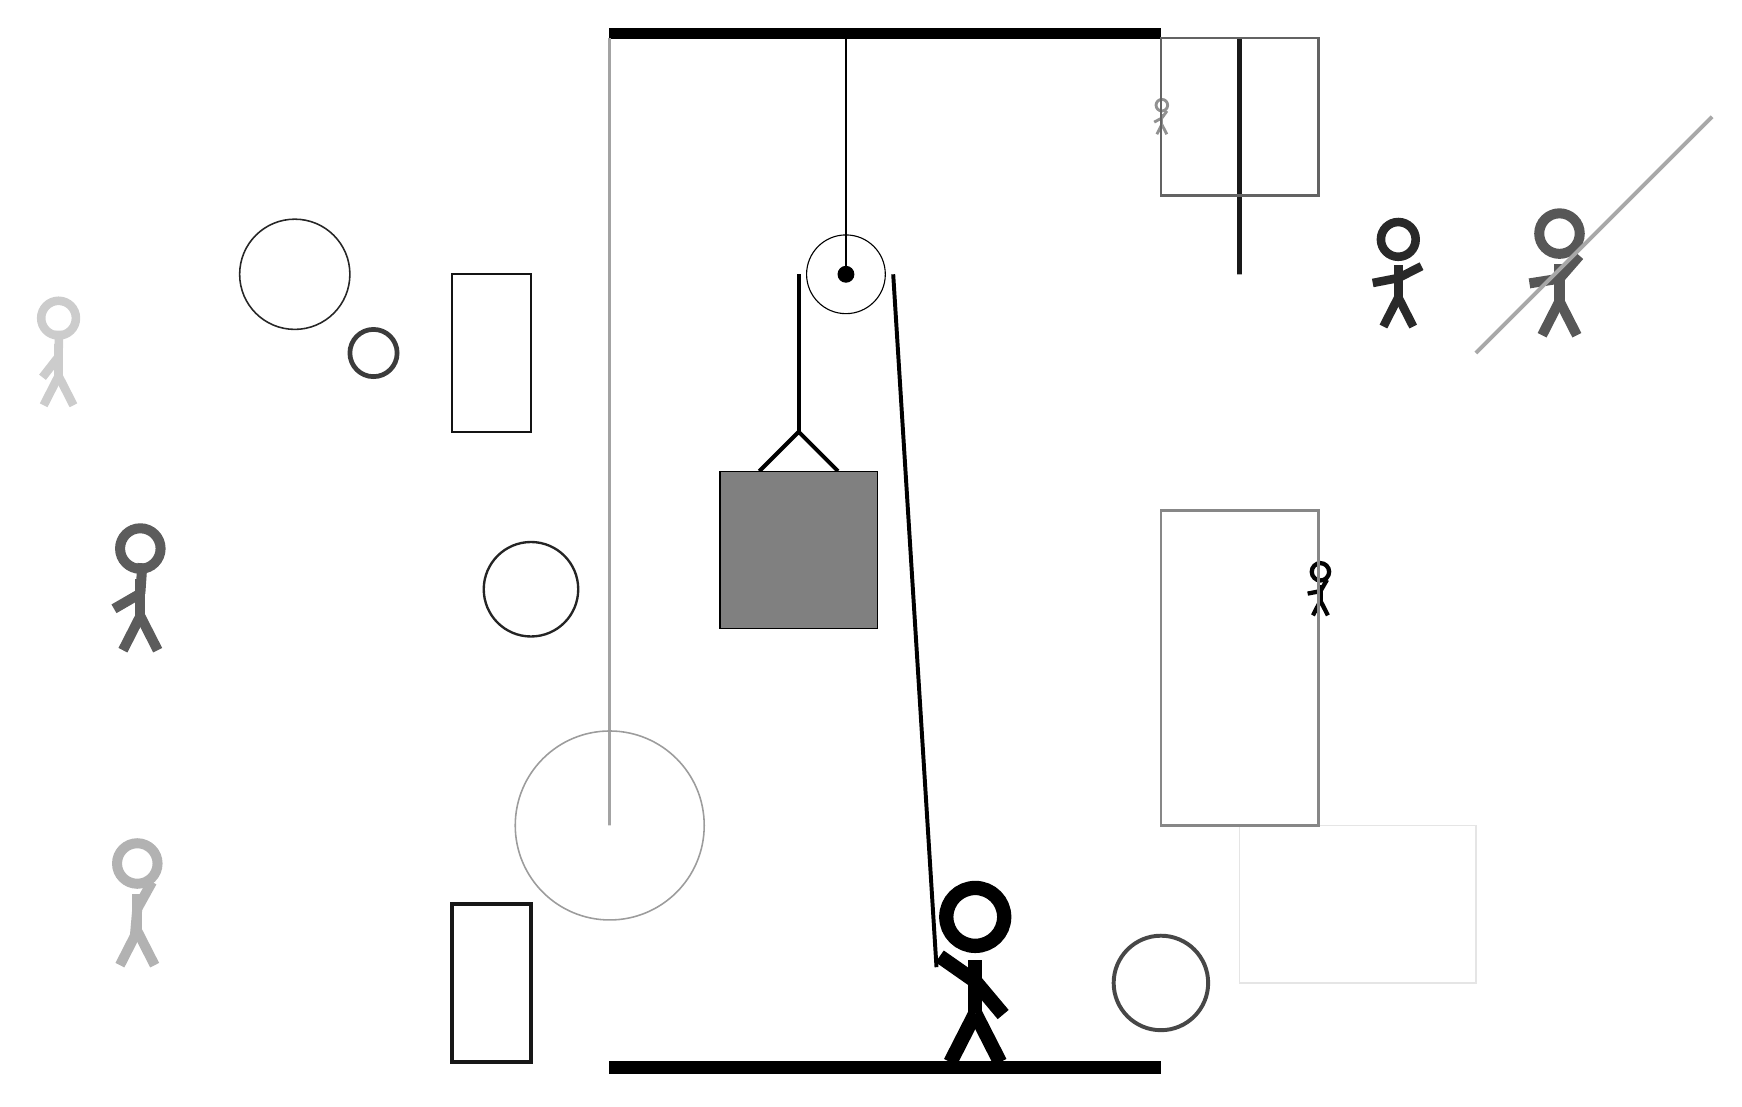
\begin{tikzpicture}
		%%%%% START %%%%%
		
		\draw[fill=black] (-2, 10) rectangle (5, 10.125);
		
		\draw (1, 7) circle (0.5);
		\draw[fill=black] (1, 7) circle (0.1);
		\draw (1, 10) -- (1, 7);
		
		\draw[line width=0.5mm] (-0.1, 4.5) -- (0.4, 5.0) -- (0.9, 4.5);
		\draw[fill=black!50] (-0.6, 4.5) rectangle (1.4, 2.5);
		
		\draw [line width=0.3mm, color=black!86](-3, 3) circle (0.6);
		
		\node[line width=0.3mm, color=black!66] at (10, 7) {\Strichmaxerl[7][9][49]};
		\node[line width=0.2mm, color=black!43] at (5, 9) {\Strichmaxerl[2][28][54]};
		\draw[line width=0.3mm, color=black!92] (-4, 5) rectangle (-3, 7);
		\draw[line width=0.5mm, color=black!91] (-3, -1) rectangle (-4, -3);
		\node[line width=0.4mm, color=black!99] at (7, 3) {\Strichmaxerl[3][11][60]};
		\draw[line width=0.5mm, color=black!34](9, 6) -- (12, 9);
		\draw[line width=0.7mm, color=black!90] (6, 10) rectangle (6, 7);
		\node[line width=0.5mm, color=black!84] at (8, 7) {\Strichmaxerl[6][11][27]};
		\draw [line width=0.5mm, color=black!72](5, -2) circle (0.6);
		\draw[line width=0.2mm, color=black!10] (6, 0) rectangle (9, -2);
		
		\draw [line width=0.6mm, color=black!77](-5, 6) circle (0.3);
		\node[line width=0.7mm, color=black!20] at (-9, 6) {\Strichmaxerl[6][52][89]};
		
		\draw[line width=0.3mm, color=black!61] (7, 8) rectangle (5, 10);
		\draw[line width=0.4mm, color=black!36] (-2, 0) rectangle (-2, 10);
		\draw [line width=0.2mm, color=black!85](-6, 7) circle (0.7);
		\node[line width=0.6mm, color=black!30] at (-8, -1) {\Strichmaxerl[7][85][61]};
		
		\draw[line width=0.3mm, color=black!47] (7, 4) rectangle (5, 0);
		\draw [line width=0.2mm, color=black!39](-2, 0) circle (1.2);
		
		\node[line width=0.5mm, color=black!64] at (-8, 3) {\Strichmaxerl[7][30][86]};
		
		\draw[line width=0.5mm] (0.4, 7) -- (0.4, 5.0);
		\centerarc[line width=0.5mm](1, 7)(0:180:0.6);
		\draw[line width=0.5mm](1.6, 7) -- (2.15, -1.8);
		
		\node at (2.6, -1.9) {\Strichmaxerl[10][-35][-50]};
		
		\draw[fill=black] (-2, -3) rectangle (5, -3.15);
		
		%%%%% END %%%%%
	\end{tikzpicture}
\end{document}